\documentclass[conference]{IEEEtran}
\usepackage[brazilian]{babel}
\usepackage[utf8]{inputenc}
\usepackage[T1]{fontenc}
\usepackage{cite}
\ifCLASSINFOpdf
  \usepackage[pdftex]{graphicx}
  % declare the path(s) where your graphic files are
  % \graphicspath{{../pdf/}{../jpeg/}}
  % and their extensions so you won't have to specify these with
  % every instance of \includegraphics
  % \DeclareGraphicsExtensions{.pdf,.jpeg,.png}
\else
  % or other class option (dvipsone, dvipdf, if not using dvips). graphicx
  % will default to the driver specified in the system graphics.cfg if no
  % driver is specified.
  \usepackage[dvips]{graphicx}
  % declare the path(s) where your graphic files are
  % \graphicspath{{../eps/}}
  % and their extensions so you won't have to specify these with
  % every instance of \includegraphics
  % \DeclareGraphicsExtensions{.eps}
\fi

\usepackage{adjustbox}
\usepackage{fancyvrb}

\usepackage[cmex10]{amsmath}
\usepackage{algorithmic}
\usepackage{array}
\usepackage{mdwmath}
\usepackage{mdwtab}
%\usepackage{eqparbox}
\usepackage[tight,footnotesize]{subfigure}
%\usepackage[caption=false]{caption}
\usepackage[font=footnotesize]{subfig}
%\usepackage{stfloats}
\usepackage{url}
\usepackage{csvsimple,longtable,booktabs}
\usepackage{pgfplots}
\usepackage{pgfplotstable}
\hyphenation{op-tical net-works semi-conduc-tor}
%\usepackage{listings}

%\lstset{language=C++,
%	basicstyle=\ttfamily,
%	keywordstyle=\color{blue}\ttfamily,
%	stringstyle=\color{red}\ttfamily,
%	commentstyle=\color{green}\ttfamily,
%	morecomment=[l][\color{magenta}]{\#}
%}

\begin{document}
\title{Programação de Alto Desempenho\\
\large Atividade 6 - Exercícios em MPI}

\author{\IEEEauthorblockN{Lucas Santana Lellis - 69618}
\IEEEauthorblockA{PPGCC - Instituto de Ciência e Tecnologia\\
	Universidade Federal de São Paulo} }

% make the title area
\maketitle

%\IEEEpeerreviewmaketitle

\section{Introdução}
Nesta atividade foram realizados alguns exercícios utilizando MPI em conjunto com OpenMP.
Cada experimento foi realizado 3 vezes, e os resultados apresentados são a média dos resultados obtidos em cada um deles, sendo calculado o speedup pela fórmula $$speedup(P) = {{\textrm{Tempo para 1 thread} }\over{\textrm{Tempo para P threads} }}$$ e a eficiência pela fórmula $$eficiencia(P) = {{speedup(P)}\over{P}}$$


Foram utilizados dois computadores, um desktop (i5-3470, 4 cores, 4 threads, 8Gb RAM DDR3) e um notebook (i5-3210M, 2 cores, 4 threads, 6Gb RAM DDR3), ambos com Fedora 25 x86\_64, kernel 4.8.8, GCC 6.2.1 e MPICH 3.2. Todos os programas foram feitos em C, com otimização -O3.


\section{Exercício I- Novidades do MPI 3}

O MPI 3 é padrão mais recente do MPI, e uma das suas maiores novidades é o suporte à sistemas de memória compartilhada, diminuindo a necessidade de utilização de pthreads ou OpenMP, assim como novidades em comunicação "One-Sided" e operações coletivas. Abaixo, algumas das mudanças mais relevantes:

\subsection{Operações Coletivas Não-bloqueantes}
Operações coletivas não bloqueantes, como as funções ``MPI\_Ibcast'' e ``MPI\_Iallreduce'' permitem uma maior sobreposição de comunicação e computação, aumentando a perfomance dos programas.

\subsection{Neighborhood Collectives}
Esse recurso permite a utilização de operações coletivas considerando uma topologia pré-definida. Assim, operações de redução e comunicação coletivas podem ser executadas de acordo com as vizinhanças de forma mais simples e direta.

\subsection{Novidades em RMA}

Foram adicionadas novas rotinas para criação de janelas, como ``MPI\_Win\_allocate'' , ``MPI\_Win\_create\_dynamic'' e ``MPI\_Win\_allocate\_shared''.

A função ``MPI\_Win\_allocate\_shared'' permite que uma janela de memória seja compartilhada entre diferentes processos em um mesmo nó usando apenas MPI, favorecendo a utilização do MPI em sistemas de memória compartilhada, e reduzindo a complexidade de implementação se comparado à aplicações hibridas (OpenMP + MPI).

Consta também a adição de operações atômicas, como ``MPI\_Get\_accumulate'', ``MPI\_Fetch\_and\_op'', e ``MPI\_Compare\_and\_swap'', além da adição de versões adicionais de Put, Get e Accumulate que retornam objetos do tipo request, desta forma podemos usar funções Test e Wait para verificar localmente se a operação terminou.

% ################################################################################
% ################################################################################

\section {Jogo da Vida}

Foram implementadas duas versões do algoritmo ``Jogo da Vida'' utilizando MPI, a primeira baseada em comunicação ponto-a-ponto, e a segunda baseada na comunicação unidirecional do MPI-2. A divisão do tabuleiro foi feita verticalmente, de forma que cada processo recebe uma porção das linhas do tabuleiro para processar.

Em ambos os exemplos, o resultado da execução do algoritmo em um tabuleiro pré-definido de tamanho 1250x1250, na Figura \ref{fig:ex02} uma representação das 10 últimas linhas e colunas do canto inferior direito após o final da execução do algoritmo.

\textit{ Obs. A implementação do algoritmo com comunicação ponto-a-ponto poderia ter sido otimizada caso fosse feito uma troca entre os ponteiros ``aux'' e ``localdata'', mas essa otimização não era possível no segundo exemplo, então teve que ser descartada para tornar a comparação entre os dois mais justa. }


\begin{figure}[!htb]
\begin{verbatim}
+------------+
|            |
|            |
|            |
|            |
|            |
|            |
|            |
|            |
|         0  |
|          0 |
|        000 |
|            |
+------------+
\end{verbatim}
\caption{Condições iniciais do teste em tabuleiro 10x10.}
\label{fig:ex02}
\end{figure}

\subsection{Comunicação ponto-a-ponto \label{sec:ex02a}}
O primeiro programa utiliza comunicações ponto-a-ponto para distribuir os dados entre os processos. Nesta abordagem, o processo 0 inicializa a matriz e envia os pedaços correspondentes para cada um dos outros processos. Durante a execução do algoritmo, as ghost zones são trocadas entre os processos por operações send e receive assíncronas. Os resultados da execução do primeiro algoritmo estão na Tabela \ref{tab:ex02a}, o número crescente de processos é distribuido igualmente entre os nós.

\begin{table}[htb!]
  \centering
	\begin{adjustbox}{max width=\linewidth}
	\begin{tabular}{llrrr}%
		\bfseries Maquinas & \bfseries Processos & \bfseries Tempo(s) & \bfseries Speedup & \bfseries Eficiencia  \\
    1 &	1	& 18.783	& 1	    & 1     \\
    1 &	4	& 11.289	& 1.663 & 0.415 \\
    2 &	2	& 15.589	& 1.204 & 0.602 \\
    2 &	4	& 16.049	& 1.170 & 0.292 \\
    2 &	8	& 30.498	& 0.615 &	0.076 \\

	\end{tabular}
	\end{adjustbox}
	\caption{\label{tab:ex02a}Avaliação do desempenho do jogo da vida com comunicação ponto-a-ponto, tabuleiro de tamanho 1250x1250.}
\end{table}

\subsection{Comunicação unidirecional \label{sec:ex02b}}
O segundo programa utiliza comunicações unidirecionais, de forma que o MPI se utiliza de operações RMA para obter ou inserir dados em janelas de comunicação abertas pelos outros processos.

Nesta abordagem a matriz é inicializada no processo 0, que então abre uma janela de compartilhamento para que os outros processos busquem pelas linhas do tabuleiro atribuidas a eles. Durante o processamento, as ghost zones são implementadas por meio de janelas compartilhadas entre os processos.


Os resultados da execução do primeiro algoritmo estão na Tabela \ref{tab:ex02b}, o número crescente de processos é distribuido igualmente entre os nós.

\begin{table}[htb!]
  \centering
	\begin{adjustbox}{max width=\linewidth}
	\begin{tabular}{llrrr}%
		\bfseries Maquinas & \bfseries Processos & \bfseries Tempo(s) & \bfseries Speedup & \bfseries Eficiencia  \\
    1	& 1 &	18.732 & 1	   & 1     \\
    1	& 4 &	12.840 & 1.458 & 0.364 \\
    2	& 2 &	19.982 & 0.937 & 0.468 \\
    2	& 4 &	19.933 & 0.939 & 0.234 \\
    2	& 8 &	43.129 & 0.434 & 0.054 \\
	\end{tabular}
	\end{adjustbox}
	\caption{\label{tab:ex02b}Avaliação do desempenho do jogo da vida com comunicação unidirecional, tabuleiro de tamanho 1250x1250.}
\end{table}

\subsection{Discussão dos resultados}
Ao analisar as tabelas \ref{tab:ex02a} e \ref{tab:ex02b} percebemos que os algoritmos com comunicação ponto-a-ponto se demonstraram muito mais eficientes, uma vez que a utilização do MPI não demonstrou nenhuma melhora no desempenho no algoritmo com comunicação unidirecional.

Além disso, como esperado, os experimentos em que os 4 processos foram atribuidos à uma só máquina obtiveram melhor resultado se comparado à divisão entre duas máquinas, pois a segunda fica limitada pela comunicação por rede ethernet.

Outra informação relevante é a baixíssima eficiência obtida ao se dividir o problema em 8 processos - em ambos os casos, essa foi a configuração que obteve o maior tempo de execução e também o menor speedup e eficiência.

Finalmente, a comparação entre as duas implementações se torna mais evidente na Tabela \ref{tab:ex02comp}, onde os tempos de execução da Tabela \ref{tab:ex02b} são divididos pelos valores da Tabela \ref{tab:ex02a}.


\begin{table}[htb!]
  \centering
	\begin{adjustbox}{max width=\linewidth}
	\begin{tabular}{llrrr}%
		\bfseries Maquinas & \bfseries Processos & \bfseries Tempo Exp. A & \bfseries Tempo Exp. B & \bfseries B / A  \\
    1	& 1 &	18.783 & 18.732 &	0.997 \\
    1	& 4 &	11.289 & 12.840 &	1.137 \\
    2	& 2 &	15.589 & 19.982 &	1.281 \\
    2	& 4 &	16.049 & 19.933 &	1.241 \\
    2	& 8 &	30.498 & 43.129 &	1.414 \\
	\end{tabular}
	\end{adjustbox}
	\caption{\label{tab:ex02comp}Comparação entre o desempenho do jogo da vida com comunicação ponto-a-ponto (Exp. A) e comunicação unidirecional (Exp. B).}
\end{table}

\section{ Programação Híbrida - MPI + OpenMP\label{sec:ex03}}
Nesse experimento, o programa descrito na seção \ref{sec:ex02a} foi adaptado para a paralelização em sistema de memória compartilhada, usando o OpenMP.
Além do que já foi mencionado na seção \ref{sec:ex02a}, a imagem foi subdividida novamente, agora distribuindo as linhas entre as threads no laço mais externo dentro da função ``evolve''.
Assim como no exercício anterior, o resultado da execução do algoritmo em um tabuleiro pré-definido de tamanho 1250x1250 também se iguala ao do algoritmo clássico, e as últimas 10 linhas e colunas são as mesmas da Figura \ref{fig:ex02}.


Foram realizados 5 experimentos ao total, variando-se o número de threads, processos, distribuindo ou não o processo entre duas máquinas - os resultados estão na Tabela \ref{tab:ex03}.

\begin{table}[htb!]
  \centering
	\begin{adjustbox}{max width=\linewidth}
	\begin{tabular}{llllrrr}%
		\bfseries Maquinas & \bfseries Proc. & \bfseries Thd./Proc. & \bfseries Total Thds & \bfseries Tempo(s) & \bfseries Speedup & \bfseries Eficiencia \\
    1	& 1	& 1	& 1	& 18.712 & 1.000 & 1.000 \\
    1	& 4	& 1	& 4	& 12.350 & 1.515 & 0.379 \\
    2	& 8	& 1	& 8	& 30.653 & 0.610 & 0.076 \\
    1	& 1	& 4	& 4	& 10.379 & 1.803 & 0.451 \\
    2	& 2	& 4	& 8	& 14.392 & 1.300 & 0.163 \\
	\end{tabular}
	\end{adjustbox}
	\caption{\label{tab:ex03}Avaliação do desempenho do jogo da vida com comunicação ponto-a-ponto e OpenMP, tabuleiro de tamanho 1250x1250.}
\end{table}

Avaliando os resultados, percebe-se um speedup positivo na maioria dos exemplos, porém, assim como no exercício anterior, quando 8 processos eram distribuidos entre as duas máquinas, a eficiência foi muito baixa, e o speedup foi menor do que 1.

Percebe-se também, que em geral a utilização do OpenMP favoreceu grandemente o desempenho se comparado ao MPI puro com número equivalente de threads. Esse resultado era esperado, pois o número de comunicações pela rede, e entre processos é mais lento que a comunicação entre as threads em um sistema de memória compartilhada.

\section{Exercício da Maratona da WSCAD}
Para esse exercício foi selecionado o problema D, que é o calculo do histograma de uma imagem. Foi feita então a paralelização do algoritmo utilizando MPI e OpenMP.  Neste programa, as linhas da imagem são divididas entre os processos, e dentro de cada processo o openmp é utilizado em duas ocasiões, por fim, uma operação de redução soma os histogramas de cada partição da imagem.

O algoritmo inicialmente realiza uma quantização dos pixels, essa operação é paralelizada com ``omp parallel for'', distribuindo os pixels entre as diferentes threads.
Em seguida, quatro laços aninhados são utilizados para contar ocorrências das 64 possíveis combinações de cores agora disponíveis, e embora o laço mais externo possua apenas quatro iterações, optei por paralelizá-lo, pois seriam utilizadas 4 threads no máximo.
Outra opção seria paralelizar o laço interno, utilizando operações de redução para acumular o valor do contador de ocorrências.

A imagem utilizada nos testes é a da Figura \ref{fig:ex04_1}, com  8960x8897 pixels - originalmente com 21MB no formato jpg, e após a conversão para PPM pelo Imagemagick passou a ter 229 MB.


\begin{figure}[!htb]
  \centering
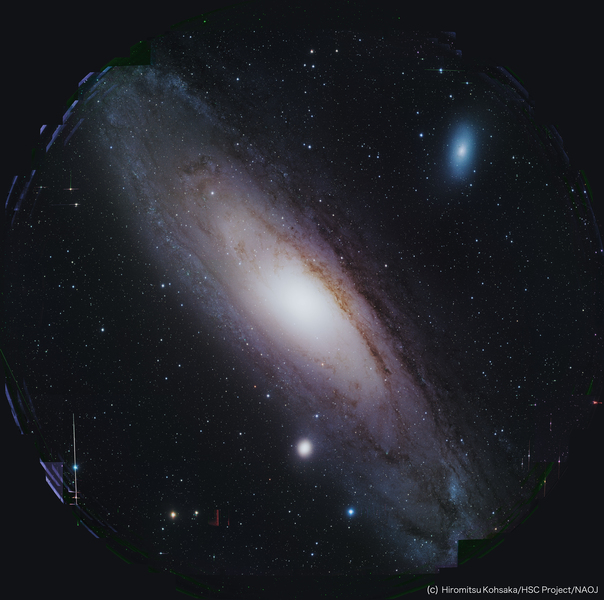
\includegraphics[width=0.4\textwidth] {small-image.jpg}
\caption{M31 - Galáxia de andrômeda (Créditos: Hiromitsu Kohsaka/HSC Project/NAOJ) - Obtido em \url{http://subarutelescope.org/Topics/2014/09/08/index.html} .}
\label{fig:ex04_1}
\end{figure}

 O resultado da execução do algoritmo foi conferido em todos os testes, e o histograma obtido é o mesmo da Figura \ref{fig:ex04_2}.

\begin{figure}[!htb]
  \begin{adjustbox}{max width=\linewidth}
	\begin{BVerbatim}
0.832 0.032 0.000 0.000 0.000 0.009 0.001 0.000 0.000 0.000 0.000 0.000
0.000 0.000 0.000 0.000 0.002 0.009 0.000 0.000 0.000 0.061 0.005 0.000
0.000 0.000 0.001 0.000 0.000 0.000 0.000 0.000 0.000 0.000 0.000 0.000
0.000 0.005 0.004 0.000 0.000 0.001 0.023 0.003 0.000 0.000 0.000 0.001
0.000 0.000 0.000 0.000 0.000 0.000 0.000 0.000 0.000 0.000 0.000 0.000
0.000 0.000 0.000 0.009
  \end{BVerbatim}
  \end{adjustbox}
\caption{Histograma da Figura \ref{fig:ex04_1}.}
\label{fig:ex04_2}
\end{figure}


Assim como na seção \ref{sec:ex03}, foram realizados 5 experimentos ao total, variando-se o número de threads, processos, distribuindo ou não o processo entre duas máquinas. Os resultados da execução do programa sobre a Figura \ref{fig:ex04_1} estão na Tabela \ref{tab:ex04}.


\begin{table}[htb!]
  \centering
	\begin{adjustbox}{max width=\linewidth}
	\begin{tabular}{llllrrr}%
		\bfseries Maquinas & \bfseries Proc. & \bfseries Thd./Proc. & \bfseries Total Thds & \bfseries Tempo(s) & \bfseries Speedup & \bfseries Eficiencia \\
    1	& 1	& 1	& 1	& 18.712 & 1.000 & 1.000 \\
    1	& 4	& 1	& 4	& 12.350 & 1.515 & 0.379 \\
    2	& 8	& 1	& 8	& 30.653 & 0.610 & 0.076 \\
    1	& 1	& 4	& 4	& 10.379 & 1.803 & 0.451 \\
    2	& 2	& 4	& 8	& 14.392 & 1.300 & 0.163 \\
	\end{tabular}
	\end{adjustbox}
	\caption{\label{tab:ex04}Avaliação do desempenho do cálculo do histograma, com comunicação ponto-a-ponto e OpenMP, para uma imagem colorida de 8960x8897 pixels.}
\end{table}

\bibliographystyle{IEEEtran}

%\bibliography{references}

\end{document}
